\chapter{Background}
The motivation behind solving chess puzzles, especially under time pressure,
is to improve one's pattern recognition abilities. It has been shown \cite{thoughtAndChoice} 
that chess players do not have a square-by-square, recollection of the chess board 
during play. Instead, they rely on interactions, and potential interactions,
of pieces in a more abstract sense. This is made strikingly clear by a chess 
player's drawing of a position from memory (Figure \ref{deGrootFigure}).
\\~\\
de Groot writes, ``the pieces themselves do not appear in the drawing: 
rather the lines of force that go out from them''. This heuristic allows expert
human players to quickly hone in on the correct moves \cite{bilalic2010mechanisms},
and significantly reduces their search space, when compared to a naive brute-force
search, which is the most common strategy for chess engines. When analysing 
positions, even the most basic chess engines are able to calculate the most 
accurate line (except some pathological cases), but they are unable to draw
similarities between different positions.

\begin{figure}[H]
    \centering
    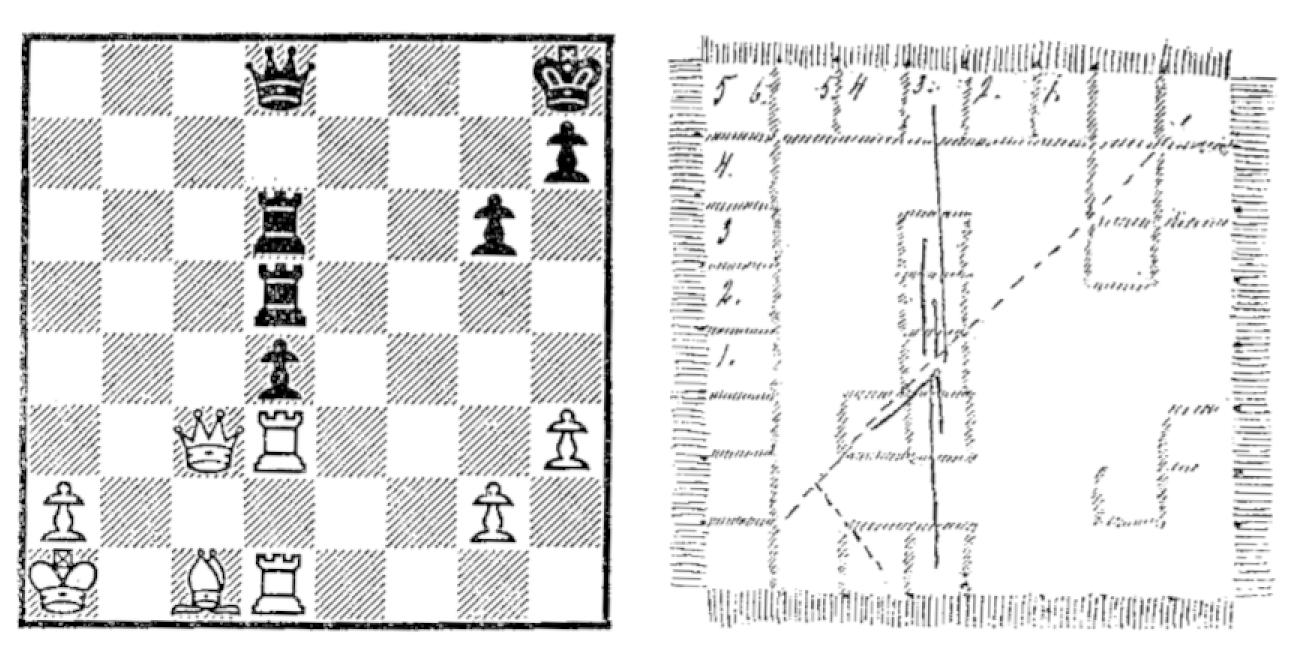
\includegraphics[width=0.9\linewidth]{background/img/deGroot.png}
    \caption{Taken from de Groot's `Thought And Choice In Chess' \cite{thoughtAndChoice}.}
    \label{deGrootFigure}
\end{figure}
\\~\\
In Figures \ref{chess1}, \ref{chess2}, 2 chess positions are shown, featuring 
\emph{back rank checkmates} -- one of the first tactical patterns that a beginner 
might learn. A castled king is forced to stay on the back rank due to the 
configuration of his men, and an opposing heavy piece exploits this weakness
by delivering checkmate. It is already non-trivial to programmatically identify
this type of tactic, as a checkmate delivered to a king on the back rank is not
necessarily a \emph{back rank checkmate}.
\\~\\
Given positions similar to ones like these, how does one draw similarities 
between the abstract relations of the heavy piece, king, and vulnerable back rank?

\begin{figure}[H]
    \begin{minipage}{0.475\textwidth}
        \centering
        \chessboard[setfen=6k1/5ppp/8/8/8/8/r4PPP/1R4K1 w - - 0 1]
        \caption{A trivial backrank checkmate, white mates with \textbf{Rb8\#}
        (TODO: Find real chess games where these positions/similar ones happened)}
        \label{chess1}
    \end{minipage}
    \hspace{0.05\textwidth}
    \begin{minipage}{0.475\textwidth}
        \centering
        \chessboard[setfen=6k1/5ppp/1p1Q4/p3p1B1/Pn4P1/1q6/1Pr4P/K6R w - - 1 2]
        \caption{White mates with \textbf{Qd8\#}.}
        \label{chess2}
    \end{minipage}
\end{figure}

\section{Chess notation}
TODO: Explain chess FEN, PGN notation. The reader is assumed to know how to play 
chess at a basic level
\\~\\
TODO: Show examples of basic puzzles/tactics in chess
\\~\\
TODO: Explain basic chessprogramming, e.g. bitboards, 0x88

\section{A language for encoding piece relationships}
In ``A description language for chess'' \cite{chessLanguage}, López-Michelone et al. 
describe a language to search across chess positions. The main features of this
language are descriptions for a chess piece attacking/defending another, 
attacking/defending a square, being located at a square, a square not being 
available for the enemy king, and the structure of white/black pawns on the board.
\\~\\
With their novel language, they are able to search a chess database for a 
pre-determined pattern, such as the \emph{Greek gift sacrifice}, defined in the language as 
``kg8, pf7, pg7, B(ph7), Nf3, Qd1, Pe5''
\footnote{This string corresponds to a black king on g8, black pawns on f7, g7, h7,
a white bishop attacking h7, a white knight on f3 (ready to deliver a check with \textbf{Ng5+},
a common motif in \emph{Greek gift sacrifices}), a white queen on d1, and finally, a
white pawn on e5 to dislodge the usual black knight on f6.}
, which returns positions such as 
the one shown in Figure \ref{chess3}. After \textbf{16...Be7 17. O-O}, Black blundered with
\textbf{17...Bxa3??}, after which, the \emph{Greek gift sacrifice} (\textbf{18. Bxh7!!}, 
shown in Figure \ref{chess4}) was employed, eventually culminating in a win for White.

\begin{figure}[H]
    \begin{minipage}{0.475\textwidth}
        \centering
        \chessboard[setfen=r1b2rk1/qp3ppp/p1n1pb2/4P3/3P4/P1BB1N2/5PPP/1R1QK2R b K - 0 16]
        \caption{\textbf{Pirc, V -- Porreca, G}, YUG-ITA m 1953, move 16.}
        \label{chess3}
    \end{minipage}
    \hspace{0.05\textwidth}
    \begin{minipage}{0.475\textwidth}
        \centering
        \chessboard[setfen=r1b2rk1/qp3ppB/p1n1p3/4P3/3P4/b1B2N2/5PPP/1R1Q1RK1 b - - 0 18]
        \caption{\textbf{Pirc, V -- Porreca, G}, YUG-ITA m 1953, move 18. Black resigned after 6 moves.}
        \label{chess4}
    \end{minipage}
\end{figure}
\\~\\
Their language is also able to deal with some light variations, as it is able
to identify the games shown in Figures \ref{chess5}, \ref{chess6}. In both of 
these positions, White has the brilliant move \textbf{1. Qh6+!!}, following with 
\textbf{2. Rh8\#} if \textbf{1...Kxh6}, and either \textbf{2. Rf7\#} or \textbf{2. Rb7+}
(leading to a quick mate) if \textbf{1...gxh6}. 
\\~\\
This pattern, whilst very rare, is undeniably identical between the 2 games. 
The unavailability of the \textbf{g6} square to the enemy king, combined with the
harmony of White's pieces leads to the same tactic in both games.

\begin{figure}[H]
    \begin{minipage}{0.475\textwidth}
        \centering
        \chessboard[setfen=2R5/4bppk/1p1p4/5R1P/4PQ2/5P2/r4q1P/7K w - - 5 50]
        \caption{\textbf{Carlsen, M -- Karjakin S}, World Chess Championship 2016, move 50.}
        \label{chess5}
    \end{minipage}
    \hspace{0.05\textwidth}
    \begin{minipage}{0.475\textwidth}
        \centering
        \chessboard[setfen=5R2/bp4pk/2n3p1/P7/P1q3bP/6P1/3Q3K/1R6 w - - 1 32]
        \caption{\textbf{Popov, N -- Novopashin, A}, URS-ch otbor 1979, move 32.}
        \label{chess6}
    \end{minipage}
\end{figure}
\\~\\
The work of López-Michelone et al. is a promising proof of concept that shows
the power of a language that allows to specify piece relationships on a more
abstract level than previously possible. The biggest drawback of their solution,
as mentioned by the authors, is the fact that this language still requires 
an expert with pre-existing extensive knowledge to encode the tactics into
their language. The authors hypothesise that automatic recognition of these 
patterns is likely some sort of neural network, which is one of the many possible
directions of this project.


\section{CQL: Chess Query Language}
The Chess Query Language (CQL), as invented by Costeff \cite{cql}, is another 
implementation of an advanced way to find chess positions in a given database.
Since its inception in 2004, it has grown and is able to support very powerful,
sometimes esoteric, queries to find predefined patterns.
\\~\\
TODO: Show examples from \url{http://www.gadycosteff.com/cql/examples/smotheredmate.html}
and \url{http://www.gadycosteff.com/cql/examples/turton.html}
\\~\\
In addition to the Costeff's CQL, there is a from-scratch clone of CQL 6.1 which includes
extra features (TODO: list some) and supports other chess variants \cite{cqli}.

\section{lichess.org puzzle database}
\url{https://lichess.org} is a popular, open-source chess website which often
publishes the games that have been played by players of all skill levels on it.
As part of this, Lichess has published over 3.6 million rated and tagged
puzzle positions \cite{lichessPuzzles}. To generate these, 300 million games
were analysed with a powerful chess engine to find critical positions in which
a move must be played to capitalise on the opponent's mistake. These puzzles
were initially tagged to 124 manually created themes \cite{lichessXML}, which
were identified by a python implementation \cite{lichessTagger}. 
\\~\\
As various users of the site solved the puzzles, and manually highlighted the
themes that they felt occured in the puzzle, the ratings and tags of the puzzle
database evolved until their current state.
\\~\\
This database is invaluable for this project, and can likely serve either as input,
or as a baseline to compare the results to.

\section{Recognition of the \emph{Greek gift sacrifice} in  chess games}
Miroslav et al. report their findings on a program \cite{middlegamePatterns}
to identify the \emph{Greek gift sacrifice} in chess middlegames
\footnote{A hard-to-quantify phase of the chess game where
most pieces are developed and the kings are positioned away from danger.}. They
found success, partly thanks to their detailed representatioon of the board, where
each square is represented by 71 binary attribites \cite{middlegamePatterns} to
encode the piece on the square and the possible squares which are reachable by
this piece. 
\\~\\
These attributes were also supplemented by 59 other binary attribites which were
devised by expert chess players, and represent the more complex, but still
quantifiable relationships \cite{middlegamePatterns}. These include open files,
control of vulnerable squares, piece activity, and so on.
\\~\\
Miroslav et al. achieved an 87.7\% classification performance on detecting whether
a position features a successful \emph{Greek gift sacrifice} on relatively 
small (<200 positions) datasets. This work is promising, but more investigation
is needed given their analysis of only one pattern with a decision tree algorithm.
Also, their program still relied on predetermined chess patterns, which introduces
bias and might miss intricate similarities between positions.

\section{A novel chess board representation for convolutional neural networks}
In Sabatelli's thesis \cite{chessCNN}, the effectiveness of neural networks to analyse whether
a chess position is winning or losing is explored, without creating specific
look-ahead algorithms. This is a very challenging task, but as part of the analysis,
the author proposed manually encoded features to a convolutional neural network (CNN)
to help identify strong patterns within the position. 
\\~\\
Some of these include an extra feature if the opponent is in check, specifying
the squares controlled by a piece exerting a pin on a different piece, centre
control, and vulnerable squares \cite{chessCNN}. These are well known heuristics that are often
taught to beginner-intermediate chess players, and the author claims that these
additional layers are ``extremely representative of the chess positions'', and
cause the CNN to outperform a naive, fully-connected neural network.
\\~\\
This work is also a promising result, as it shows that these chess patterns,
albeit manually quantified, are valuable for an algorithm when analysing a given
chess position.

\section{Chess moves as kernels for texture classifier}
In this study, Turker et al. propose novel kernels for efficient feature extraction
in the task of texture detection \cite{chessKernel}. These 5x5 kernels are
directly based on the move a rook, bishop, knight, and their combinations. 
\\~\\
Whilst not directly applicable to the context of chess puzzle analysis, this work
shows that it may be possible to include these kernels in an CNN-based analysis
of the chess position. It would be interesting to apply to the other CNN chess work
(e.g. Sabatelli's thesis \cite{chessCNN}, discussed above) and analyse its
effect on the success of the technique.

\section{TODO: Research + summarise more papers}

\section{Ethical discussion}
This project has few, if any, ethical considerations that need to be made. The
biggest concern is the source of the large datasets that may be used in this 
project, namely, the Lichess puzzle database \cite{lichessPuzzles}. However,
this database, along with all Lichess games is released under the 
Creative Commons CC0 license -- meaning there is no restriction in its use.
\\~\\
Each puzzle in this database contains a link to the game from which it was
extracted, and this contains a Lichess username, which is deanonymising. In
the initial data processing stage, these links are going to be removed, as
they are unnecessary for the goals of the project.
\\~\\
Another concern is the use of, and reference to specific chess games and the
players in them, and various chess compositions\footnote{An artificially 
created position to showcase a uniquely challenging, rare, or otherwise interesting
theme.} with their authors. Other than proper reference to the creators of the game or
composition, there are no other considerations to be made.